\documentclass[12pt, twoside, a4paper, DIV12, BCOR16mm]{scrartcl}

\usepackage[english, ngerman]{babel}
\usepackage{graphicx, fancyhdr, lastpage, listings, wasysym, 
            bibgerm, comment, changebar} 

\usepackage[utf8]{inputenc}
\usepackage[T1]{fontenc}

\usepackage{listing}
\lstset{
  literate={ö}{{\"o}}1
           {Ö}{{\"O}}1
           {ä}{{\"a}}1
           {Ä}{{\"A}}1
           {ü}{{\"u}}1
           {Ü}{{\"U}}1
           {ß}{{ss}}1
}

\lstset{ %
language=c,                % choose the language of the code
basicstyle=\footnotesize,       % the size of the fonts that are used for the code
numbers=left,                   % where to put the line-numbers
numberstyle=\tiny,      % the size of the fonts that are used for the line-numbers
stepnumber=1,                   % the step between two line-numbers. If it's 1 each line 
                                % will be numbered
numbersep=5pt,                  % how far the line-numbers are from the code
backgroundcolor=\color{white},  % choose the background color. You must add \usepackage{color}
showspaces=false,               % show spaces adding particular underscores
showstringspaces=false,         % underline spaces within strings
frame=single,	                % adds a frame around the code
showtabs=false,                 % show tabs within strings adding particular underscores
tabsize=2,	                	% sets default tabsize to 2 spaces
captionpos=none,                   % sets the caption-position to bottom
breaklines=true,                % sets automatic line breaking
breakatwhitespace=false,        % sets if automatic breaks should only happen at whitespace
title=\lstname,                 % show the filename of files included with \lstinputlisting;
                                % also try caption instead of title
escapeinside={\#}{\ },         % if you want to add a comment within your code
morekeywords={*,...}            % if you want to add more keywords to the set
}
\usepackage{framed,shadow}

\usepackage{ae} 
\usepackage[
pdftitle={Systemprogrammierung Dokumentation},
bookmarks=true,
bookmarksnumbered=true, % Verwendete Bookmarks anzeigen
colorlinks,   % Farbige Links
linkcolor=black,
urlcolor=blue,
citecolor=black]{hyperref}
%\usepackage[dvips]{thumbpdf}

\pagestyle{fancy}

\setlength{\parindent}{0pt}  

\setlength{\textheight}{225mm}
\setlength{\headheight}{13mm}
\setlength{\topskip}{10mm}

\setcounter{tocdepth}{3}

\usepackage{color}
\definecolor{hellgrau}{gray}{0.9}
\definecolor{shadecolor}{gray}{0.9}

\newcommand{\ia}{i.\,Allg.\ }
\newcommand{\dht}{d.\,h.\ }
\newcommand{\ua}{u.\,a.\ }
\newcommand{\so}{s.\,o.\ }
\newcommand{\zb}{z.\,B.\ }
\newcommand{\zbdp}{z.\,B.:\ }
\newcommand{\idr}{i.\,d.\,R.\ }
\newcommand{\zt}{z.\,T.\ } 
\newcommand{\zz}{z.\,Zt.\ } 
\newcommand{\igs}{i.\,Ggs.\ } 

\newcommand{\code}[1]{\texttt{#1}}

\newcommand{\codeo}[2]{
\begin{shaded}
\vspace*{-2ex}
\begin{program}
\begin{leftbar}
                \label{def:#1}
                \rm #2
\end{leftbar}
\end{program}
\vspace*{-2ex}
\end{shaded}
}

\newcommand{\svs}{\vspace*{0.5ex}} 
\newcommand{\myrule}{\ \vspace{1ex} \\ \hrule} 
\newcommand{\figref}[1]{Abb.~\ref{#1}} 
\newcommand{\secref}[1]{Abschnitt~\ref{#1}} 
\newcommand{\mymargin}[1]{\marginpar{\raggedright \footnotesize \sffamily #1}} 

\renewcommand{\topfraction}{0.95}
\renewcommand{\bottomfraction}{0.95}

\newenvironment{trilist}{
    \renewcommand{\labelitemi}{\(\triangleright\)}
    \renewcommand{\labelitemii}{{\bfseries -}}
    \setlength{\partopsep}{0ex plus .5ex minus .5ex} 
    \setlength{\topsep}{-1ex plus .5ex minus .5ex} 
    \setlength{\parskip}{1.2ex plus .5ex minus .5ex}
    \setlength{\itemsep}{0pt plus .5ex minus .5ex}
    \setlength{\parsep}{0pt plus .5ex minus .5ex} 
    \begin{itemize}
    }
   {\end{itemize}}


\begin{document} 

%Titelseite
\begin{titlepage}
\sffamily
\setlength{\tabcolsep}{0mm}
\begin{tabular*}{\textwidth}{l@{\extracolsep\fill}r} 

%\hspace{-0.4cm}
%
\includegraphics[width=6cm]{Bilder/logo_welle_en}  % Englische Version des Logos 

\includegraphics[width=5cm]{Bilder/logo_welle_de} % Deutsche Version des Logos

  &
\raisebox{3mm}{
	\begin{tabular}{r}
%\rule{0cm}{0.5cm}
Studiengang Angewandte Informatik\\[0.5mm]
Fakultät Elektrotechnik und Informatik \\
\end{tabular}}
\end{tabular*}
\setlength{\tabcolsep}{6pt}

\vspace*{4cm}
\begin{center}
\textbf{\Large{Dokumentation Gruppe 10}}\\
\vspace*{1cm}
\textbf{\LARGE{Systemprogrammierung}}\\
\vspace*{2cm}
%\large{zur Erlangung des akademischen Grades}\\[2mm]
%\large{Master of Science der Informatik}\\
\end{center}

%\vfill
\vspace{1cm}
\begin{center}

	vorgelegt von:\\[5mm]
	{\Large Frank Klameth} \\
	20688 \\
	frank.klameth@hs-weingarten.de \\[5mm]
	{\Large Simon Westphahl} \\
	20146 \\
	simon.westphahl@hs-weingarten.de \\[5mm]
	{\Large Michael Wydler} \\
	20168 \\
	michael.wydler@hs-weingarten.de \\[5mm]
    \today \\[3cm]
\end{center}

\end{titlepage}

\newpage


\tableofcontents 

\section{Client}
Der Client stellt eine Verbindung zum Server her. Es werden bein starten des Client die Server- und Logindaten angegeben.

\subsection{Module}
\begin{itemize}
	\item Login
	\item Benutzeroberfläche (GUI)
	\item Live-Agent
	\item Listener-Thread
	\item Netzwerkkommunikation
	\begin{itemize}
		\item Struct vor Senden Serialisieren
		\item Nach Empfang wieder umwandeln
	\end{itemize}
\end{itemize}

\subsection{Programmstart}
Das Programm wird aus der Konsole gestartet. Es müssen folgende Parameter angegeben werden:
\begin{itemize}
	\item Servername oder IP (Servername wird in IP umgewandelt)
	\item Port
	\item Benutzername
	\item Rolle
\end{itemize}

Dabei können Benutzername und Rolle frei gewählt werden. Ist der Benutzername schon vergeben, wird ... . Ist die angegebene Rolle schon belegt, wird der Benutzer automatisch als Student eingetragen.

\paragraph{Beispiel:}
\code{> ./client 127.0.0.1 8080 michael student}

\subsection{Strukturen (intern)}
\subsubsection{Benutzerrollen}
\begin{lstlisting}
enum ROLE {
    Dozent = 1
    Tutor = 2
    Student = 3
};
\end{lstlisting}

\subsubsection{Schreib- und Leserecht}
Als Datentyp wird \code{uint8\_t} verwendet.
\begin{itemize}
	\item Modify 0 = nur lesend
	\item Modify 1 = schreibzugriff (exclusiv)
\end{itemize}

\subsection{Abläufe \label{Abläufe}}

\subsubsection{Programmstart}
\begin{lstlisting}
# Start mit Parameter (Server-IP, Port, Username, Rolle)
# Socket für Netzwerkkommunikation öffnen
# Logindaten (Username und gewünschte Rolle) an Server senden
# Login erfolgreich?
    # wenn NEIN: 
        # Fehlermeldung ausgeben
        # Kill: Client
    # wenn JA:
        # Userdaten und -rechte speichern (ID, Name, Rechte)
# Mutex für lokalen Tafelzugriff initialisieren (gesperrt)
# Initialisiere lokale Tafel
# Starte Command-Thread
# Starte Live-Agent
# Starte GUI
# Starte Listener-Thread
# Starte Trigger für Live-Agent
    # Mutex-Down für lokale Tafel
    # Fordert aktuellen Tafelinhalt an
    # Mutex-Up
\end{lstlisting}

\subsubsection{Command-Thread}
\begin{lstlisting}
> quit (Client beenden)
    # Sende Befehl "quit" an den Server
    # Mutex-Down für lokale Tafel
    # Beende Trigger für Live-Agent
    # Kill: Listener-Thread
    # Kill: GUI
    # Kill: Live-Agent
    # Kill: Command-Thread
    # Lösche lokale Tafel
    # Lösche Mutex für Tafelzugriff

> request (Schreibrecht anfordern)
    # Ist Client Student?
        # Wenn JA:
            # Sende Befehl "request" an den Server
    # Ist Client Dozent?
        # Wenn JA:
            # Dialog ob Benutzer schreibrecht bekommen soll
            # Sende Antwort an Server
    # Schreibrecht erteilt?
        # Wenn JA:
            # Deaktiviere Button 'Schreibrecht anfordern'
            # Aktiviere Button 'Schreibrecht abgeben'
            # Schreibrecht auf lokale Tafel gewähren
        # Wenn NEIN:
            # Hinweis das Anfrage abgeleht wurde.

> shutdown (System beenden)
    # Ist Client Dozent?
        # Wenn JA:
            # Sende Befehl "shutdown" an den Server

> release (Schreibrecht abgeben)
    # Ist Client Tutor?
        # Wenn JA:
            # Sende Befehl "release" an den Server

> acquire (Schreibrecht entziehen)
    # Ist Client Dozent?
        # Wenn JA:
            # Sende Befehl "acquire" an den Server

> clear (Tafel löschen)
    # Hat Client Schreibrechte?
        # Wenn JA:
            # Sende Befehl "clear" an den Server
\end{lstlisting}

\subsubsection{Live-Agent}
\begin{lstlisting}
> modify (Tafel ändern)
    # Hat Client schreibrecht?
        # Wenn JA:
            # Mutex-Down für lokale Tafel
            # Ist Tafel voll?
                # Wenn JA:
                    # Fehlermeldung
                # Wenn NEIN:
                    # Schreibe Änderung in lokale Tafel
            # Mutex-Up
            # Trigger für Tafel starten.
    # Trigger für Tafel sendet dann die Daten in bestimmten Intervallen.
    # Trigger abgelaufen?
        # Wenn JA:
            # Mutex-Down für lokale Tafel
            # Sende Tafel an Server
            # Erfolgreiche Sendung?
                # Wenn NEIN:
                    # Tafel nochmals senden
            # Mutex-Up
\end{lstlisting}

\subsubsection{GUI}
\begin{lstlisting}
# // Tafel wird als GtkTextView gespeichert.
# GtkTextBuffer *gtkbuf = gtk_text_view_get_buffer(textview);

# GtkTextIter startIter, endIter;
# char *mybuf;

# gtk_text_buffer_get_start_iter(gtkbuf, &startIter);
# gtk_text_buffer_get_end_iter(gtkbuf, &endIter);

# // Speichern in char*
# mybuf = gtk_text_buffer_get_text(gtkbuf, &startIter, &endIter, FALSE);

# // Tafel leeren
# gtk_text_buffer_set_text(gtkbuf, "", -1);

# // Tafel wieder befüllen
# gtk_text_buffer_set_text(gtkbuf, mybuf, -1);
\end{lstlisting}

\subsubsection{Listener-Thread}
\begin{lstlisting}
# Wartet auf Nachrichten vom Server (Broadcasting-Thread)
# Aktuallisierung der lokalen Tafel und der Statusinformationen.

> board_modified (Tafel-Update)
    # Mutex-Down für lokale Tafel
    # Tafel aktuallisieren
    # Mutex-Up

> states_changed (Statusänderung)
    # GUI-Informationen aktuallisieren

> my_state_changed (eigene Rechte bekommen/entzogen)
    # Schreibrecht erhalten?
        # Wenn JA:
            # Button "Schreibrecht anfordern" deaktivieren
            # Tafel editierbar setzten
    # Schreibrecht abgegeben/entzogen?
        # Wenn JA:
            # Tafel nicht-editierbar setzten
            # Button "Schreibrecht anfordern" aktivieren
\end{lstlisting}

\subsection{Tafel-Trigger}
Wenn auf die Tafel geschrieben wird, dann wird ein Timeout-Signal gestartet. Wenn dieses abgelaufen ist, wird die Tafel an den Server gesendet und somit an alle Clients verteilt.
Bei jeder Änderung wird der Timeout zurückgesetzt. Wenn der Timeout 5x zurückgesetzt wurde, dann wird die Tafel dennoch zum Server gesendet und der Timeout-Counter zurückgesetzt.
\begin{lstlisting}
# Tafel wird geändert
    # Timeout (200ms) wird (neu) gestartet
    # Timeout-Counter +1
    # Timeout abgelaufen oder Timeout-Counter = 3?
        # Wenn JA:
            # Mutex-Down für lokale Tafel
            # Tafel an Server senden
            # Timeout-Counter = 0
            # Mutex-Up
\end{lstlisting}


\section{Server}

\subsection{Programmabläufe}

\subsubsection{Hauptprogramm}
\myfigure{Ablauf Hauptprogramm}{ablaeufe/server/server_ablauf.pdf}{0.5}

\subsubsection{Login-Thread}
\myfigure{Ablauf Login-Thread}{ablaeufe/server/login_thread_ablauf.pdf}{0.5}

\subsubsection{Client-Thread}
\myfigure{Ablauf Client-Thread}{ablaeufe/server/client_thread_ablauf.pdf}{0.35}

\subsubsection{Broadcasting-Agent}
\myfigure{Ablauf Broadcasting-Agent}{ablaeufe/server/broadcasting_thread_ablauf.pdf}{0.5}

\subsection{Funktionshierarchie}
\myfigure{Funktionshierarchie Server}{hierarchie/server.pdf}{0.45}

\subsection{Modulhierarchie}
\myfigure{Modulhierarchie Server}{module/server/server_module.pdf}{0.65}

\subsection{Quellcode}
Der Quellcode ist auf der CD zu finden.

\section{Netzwerk}

\subsection{Allgemeine Definitionen}
\subsubsection{Datentypen}
Um hohe portabliltät zu gewährleisten verwenden wir nur sichere Datentypen.
Insbesondere gilt dies für Zahlen. Statt den Datentypen short, int, long verwenden
wir (u)int8\_t, (u)int16\_t, ....\\
Außerdem sollten immer Funktionen mit Längenbegrenzung benutzt werden, 
um Buffer-Overflows zu vermeiden.

\begin{figure}[ht!]
 \centering
 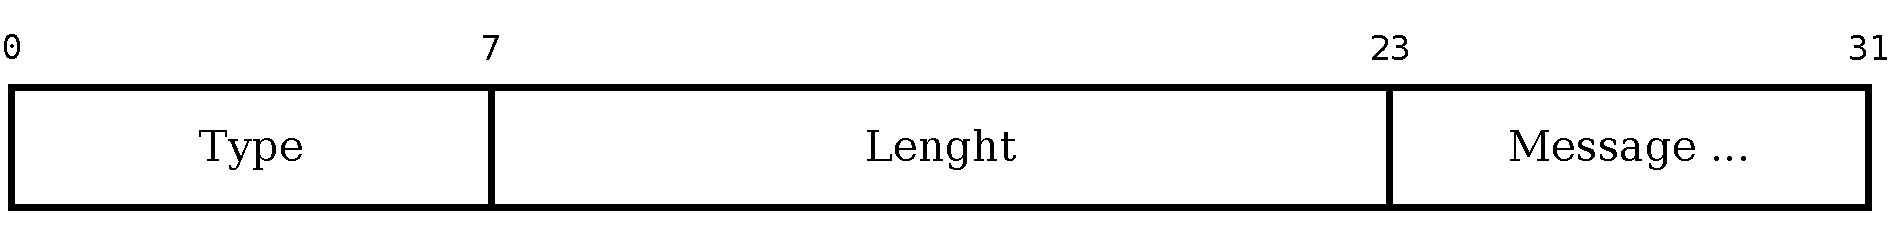
\includegraphics[width=\textwidth,keepaspectratio=true]{Bilder/header.pdf}
 \caption{Header}
 \label{Header}
\end{figure}

\subsubsection{Serialisierung}
Alle structs werden zum senden serialisiert in ein char-Array. \\
Der Server deserialisiert diesen String wieder.

\begin{lstlisting}
// PSEUDOCODE!
struct login_data {
    char name[50];
    uint8_t role;
}

// BUFFER
char buf[sizeof(login_data);

// SERIALISIEREN
strncpy(buf, login_data, sizeof(buf));

// DESERIALISIEREN
strncpy(login_data, buf, sizeof(login_data));
\end{lstlisting}

\subsubsection{Benutzerrollen}
\begin{lstlisting}
enum ROLE {
    Dozent = 1
    Tutor = 2
    Student = 3
};
\end{lstlisting}

\subsubsection{Schreib- und Leserecht}
Als Datentyp wird \code{uint8\_t} verwendet.
\begin{itemize}
	\item Modify 0 = nur lesend
	\item Modify 1 = schreibzugriff (exclusiv)
\end{itemize}

\subsubsection{Message-Types}
\begin{lstlisting}
enum M_TYPES {
    Login = 1,
    Quit, /*** eigentlich nicht nötig; Client bzw. Server */
          /*** schließt Verbindung einfach */
    Request,
    Shutdown,
    Release,
    Aquire,
    Modify,
    Clear,
    Status,
};
\end{lstlisting}

\subsection{Kommunikationsablauf}
Dieser Abschnitt spezifiziert den Austausch der einzelnen Datenstrukturen
über das Netzwerk.

Für die Beschreibung des Aufbaus der einzelnen Pakete: 
> siehe Abschnitt Datenstrukturen

\subsubsection{Login}
\begin{lstlisting}
Login       >>>
            <<<     Login
\end{lstlisting}

\subsubsection{Quit}
\begin{lstlisting}
*** eigentlich nicht nötig; Client bzw. Server schließt Verbindung einfach ***
\end{lstlisting}

\subsubsection{Request}
\begin{lstlisting}
Request     >>>
            <<<     Request (an Dozent)
# Bei Zustimmung des Dozenten die Schreibrechte abzugeben
Status      >>>
            <<<     Status (an anfragenden Client: Schreibrechte)
            <<<     Status (an alle Anderen: Tutor +1)
\end{lstlisting}

\subsubsection{Shutdown}
\begin{lstlisting}
Shutdown    >>>     (Server schließt alle Verbindungen)
\end{lstlisting}

\subsubsection{Release}
\begin{lstlisting}
Release     >>>
            <<<     Status (an releasing Client: nur Leserechte)
            <<<     Status (an Dozent: Schreibrechte)
            <<<     Status (an alle Anderen: Tutoren -1)
\end{lstlisting}

\subsubsection{Aquire}
\begin{lstlisting}
Aquire      >>>
            <<<     Status (an Client der aktuell schreibberechtig ist: nur lesend)
            <<<     Status (an Dozent: Schreibrechte)
            <<<     Status (an alle Anderen: Tutoren -1)
\end{lstlisting}

\subsubsection{Modify}
\begin{lstlisting}
Modify      >>>
            <<<     Modify (Änderungen an alle Clients verteilen)
\end{lstlisting}

\subsubsection{Clear}
\begin{lstlisting}
Clear       >>>
            <<<     Clear (an alle Clients: Tafel wurde gelöscht)
\end{lstlisting}

\subsubsection{Status}
\begin{lstlisting}
*** Ein eigener Status-Befehl existiert nicht. Status-Nachrichten
*** dienen als Bestätigung für bestimmte Befehle an den Client
*** und als Update für den Client-Status.
*** Für die Verwendung: siehe andere Befehle
\end{lstlisting}

\subsection{Datenstrukturen}
\begin{lstlisting}
#pragma pack(1)
struct HEADER {
    uint16_t size; /* Gesamtgröße in Bytes */
    uint8_t type; /* Wert aus M_TYPES */
};


/*
 * Packet:  Login
 *
 * Beschreibung:
 * Login-Versuch von Client bzw. Antwort von Server auf Login von Client.
 *
 *      >>> Richtung: Client > Server
 *      + "client_name" MUSS gesetzt und 0-terminiert sein und
 *        ist auf 25 Zeichen (inkl. O-Byte) begrenzt
 *      + "role" SOLLTE gesetzt sein, kann aber in jedem Fall vom
 *        Server geändert werden
 *
 *      >>> Richtung: Server > Client
 *      + "client_name" KANN gesetzt sein
 *      + wenn vorhanden muss dieser 0-terminiert sein und
 *        ist auf 25 Zeichen (inkl. 0-Byte) begrenzt
 *      + "role" MUSS gesetzt sein und MUSS vom Client respektiert werden
 *      + im Fehlerfall ist role == 0
 */
struct LOGIN {
    struct NET_HEADER header;
    char[25] client_name;
    uint8_t role; /* Wert aus ROLE */
};


/*
 * Packet:  Quit
 *
 * Beschreibung:
 * *** eigentlich nicht nötig; Client bzw. Server 
 * *** schließt Verbindung einfach
 *
 *      >>> Richtung: Server > Client
 *      + Keine Nutzdaten/Payload
 *      + Message Type in header ausreichend (kein "Payload Struct")
 */


/*
 * Packet:  Request
 *
 * Beschreibung:
 * Client fordert Schreibrechte an bzw. Anfrage an Dozent für Schreibrechte
 *
 *      >>> Richtung: Client > Server
 *      + "cid" wird nicht berücksichtigt
 *      + "client_name" KANN gesetzt sein
 *      + "client_name" muss 0-terminiert sein und ist auf 25 Zeichen
 *        begrenzt (inkl. 0-Byte)
 *
 *      >>> Richtung: Server > Client
 *      + "cid" MUSS gesetzt sein
 *      + "client_name" MUSS gesetzt sein
 *      + "client_name" MUSS 0-terminiert sein und ist auf 25 Zeichen
 *        begrenzt (inkl. 0-Byte)
 */
struct REQUEST {
    struct NET_HEADER header;
    uint8_t cid;
    char client_name[25];
};


/* 
 * Packet:  Shutdown
 *
 * Beschreibung:
 * System komplett beenden
 *
 *      >>> Richtung: Client > Server
 *      + Keine Nutzdaten/Payload
 *      + Message Type in header ausreichend (kein "Payload Struct")
 */


/*
 * Packet:  Release
 *
 * Beschreibung:
 * Schreibrechte an Dozent zurückgeben
 *
 *      >>> Richtung: Client > Server
 *      + Keine Nutzdaten/Payload
 *      + Message Type in header ausreichend (kein "Payload Struct")
 */


/*
 * Packet:  Aquire
 *
 * Beschreibung:
 * Aktuellem Benutzer Schreibrechte entziehen
 *
 *      >>> Richtung: Client > Server
 *      + Keine Nutzdaten/Payload
 *      + Message Type in header ausreichend (kein "Payload Struct")
 *
 */


/*
 * Packet:  Modify
 *
 * Beschreibung:
 * Änderungen an der Tafel übertragen
 *
 *		>>> Richtung: Client > Server
 *      + "cid" MUSS gesetzt sein
 *      + "board" MUSS gesetzt sein, ist 0-terminiert und max. 1200 Zeichen (inklusive 0-Byte)
 *
 *      >>> Richtung: Server > Client
 *      + "cid" wird nicht berücksichtigt
 *      + "board" MUSS gesetzt sein, ist 0-terminiert und max. 1200 Zeichen (inklusive 0-Byte)
 */
struct MODIFY {
    struct NET_HEADER header;
    uint8_t cid;
    char board[1200];
};


/*
 * Packet:  Clear
 *
 * Beschreibung:
 * Löschen des Tafelinhalts
 *
 *      >>> Richtung: Client > Server
 *      + Keine Nutzdaten/Payload
 *      + Message Type in header ausreichend (kein "Payload Struct")
 */


/*
 * Packet:  Status
 *
 * Beschreibung:
 * Änderung des Status im Server bzw. Client
 *
 *      Richtung: Client > Server (als Antwort auf 'Request'
 *      + "client_name" KANN gesetzt sein (vom Server nicht berücksichtigt)
 *      + "cid" MUSS gesetzt sein
 *      + restliche Elemente KÖNNEN gesetzt sein,
 *        aber vom Server nicht weiter berücksichtigt
 *
 *      Richtung: Server > Client
 *      + "client_name" MUSS gesetzt sein
 *      + "role" KANN gesetzt sein
 *      + "cid" KANN gesetzt sein
 *      + "write" MUSS entweder 1 = schreibender, oder 0 = lesender
 *        Zugriff sein
 *      + "nof_doz" (Anzahl angemeldeter Dozenten) KANN gesetzt sein
 *        und ist entweder 0 oder 1 (nicht mehr als 1 Dozent möglich)
 *      + "nof_tut" (Anzahl Tutoren) KANN gesetzt sein und ist
 *        entweder 0 oder 1 (Student ist nur Tutor, wenn er schreibrechte hat)
 *      + "nof_std" (Anzahl angemeldeter Studenten) KANN gesetzt sein
 */
struct STATUS {
    struct NET_HEADER header;
    char client_name[25];
    uint8_t role;
    uint32_t cid;
    unit8_t write;
    uint8_t nof_doz;
    uint8_t nof_tut
    uint32_t nof_std;
}

#pragma pack(0)
\end{lstlisting}


\end{document} 
